\documentclass[11pt]{article}
%Gummi|065|=)
\usepackage[utf8]{inputenc}
\usepackage{graphicx}

\graphicspath{ {./images/} }

\title{\textbf{What is CMMI?}}

\author{Cengiz Önkal 21706071} 
\date{}

\begin{document}

\maketitle

\section{What is CMMI ?}
The Capability Maturity Model Integration (CMMI) is a process and behavioral model that helps organizations streamline process improvement and encourage productive, efficient behaviors that decrease risks in software, product and service development.

The CMMI was developed by the Software Engineering Institute at Carnegie Mellon University as a process improvement tool for projects, divisions or organizations. The DoD and U.S. Government helped develop the CMMI, which is a common requirement for DoD and U.S. Government software development contracts. The CMMI is currently administered by the CMMI Institute, which was purchased by the ISACA in 2016.\cite{cio}

\section{How is CMMI Works ?}
The CMMI model breaks down organizational maturity into five levels. For businesses that embrace CMMI, the goal is to raise the organization up to Level 5, the “optimizing” maturity level. Once businesses reach this level, they aren’t done with the CMMI. Instead, they focus on maintenance and regular improvements.  

CMMI’s five Maturity Levels are:
\begin{enumerate}
\item \textbf{Initial}: Processes are viewed as unpredictable and reactive. At this stage, “work gets completed but it’s often delayed and over budget.” This is the worst stage a business can find itself in — an unpredictable environment that increases risk and inefficiency.
\item \textbf{Managed}: There’s a level of project management achieved. Projects are “planned, performed, measured and controlled” at this level, but there are still a lot of issues to address.
\item \textbf{Defined}: At this stage, organizations are more proactive than reactive. There’s a set of “organization-wide standards” to “provide guidance across projects, programs and portfolios.” Businesses understand their shortcomings, how to address them and what the goal is for improvement.

\item \textbf{Quantitatively managed}: This stage is more measured and controlled. The organization is working off quantitative data to determine predictable processes that align with stakeholder needs. The business is ahead of risks, with more data-driven insight into process deficiencies.

\item \textbf{Optimizing}: Here, an organization’s processes are stable and flexible. At this final stage, an organization will be in constant state of improving and responding to changes or other opportunities. The organization is stable, which allows for more “agility and innovation,” in a predictable environment.

\end{enumerate}


\begin{figure}[htp]
\centering
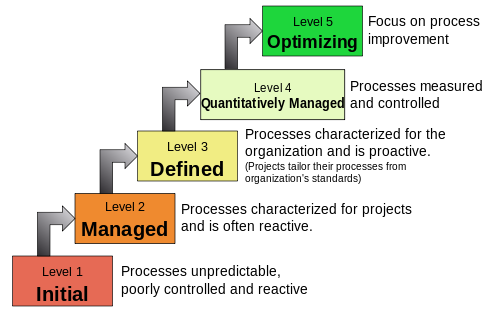
\includegraphics[scale=0.6]{images/CMMI.png}
\caption{CMMI Model}
\label{}
\end{figure}

\section{Why CMMI is Important}
CMMI is a proven process model that improves organizations' productivity, reduces cost and increases product quality.

\bibliographystyle{unsrt}
\bibliography{references}
\end{document}

